%!TEX program = xelatex

\documentclass[a4paper, openany, oneside]{memoir}
\usepackage[no-math]{fontspec}
\usepackage{pgfplots}
\pgfplotsset{compat=newest}
\usepackage{commath}
\usepackage{mathtools}
\usepackage{amssymb}
\usepackage{amsthm}
\usepackage{booktabs}
\usepackage{mathtools}
\usepackage{xcolor}
\usepackage[separate-uncertainty=true, per-mode=symbol]{siunitx}
\usepackage[noabbrev, capitalize]{cleveref}
\usepackage{listings}
\usepackage[american inductor, european resistor]{circuitikz}
\usepackage{amsmath}
\usepackage{amsfonts}
\usepackage{ifxetex}
\usepackage[dutch,english]{babel}
\usepackage[backend=bibtexu,texencoding=utf8,bibencoding=utf8,style=ieee,sortlocale=en_GB,language=auto]{biblatex}
\usepackage[strict,autostyle]{csquotes}
\usepackage{parskip}
\usepackage{import}
\usepackage{standalone}
\usepackage{hyperref}
%\usepackage[toc,title,titletoc]{appendix}

\ifxetex{} % Fonts laden in het geval dat je met Xetex compiled
    \usepackage{fontspec}
    \defaultfontfeatures{Ligatures=TeX} % To support LaTeX quoting style
    \setromanfont{Palatino Linotype} % Tover ergens in Font mapje in root.
    \setmonofont{Source Code Pro}
\else % Terug val in standaard pdflatex tool chain. Geen ondersteuning voor OTT fonts
    \usepackage[T1]{fontenc}
    \usepackage[utf8]{inputenc}
\fi
\newcommand{\references}[1]{\begin{flushright}{#1}\end{flushright}}
\renewcommand{\vec}[1]{\boldsymbol{\mathbf{#1}}}
\newcommand{\uvec}[1]{\boldsymbol{\hat{\vec{#1}}}}
\newcommand{\mat}[1]{\boldsymbol{\mathbf{#1}}}
\newcommand{\fasor}[1]{\boldsymbol{\tilde{\vec{#1}}}}
\newcommand{\cmplx}[0]{\mathrm{j}}
\renewcommand{\Re}[0]{\operatorname{Re}}
\newcommand{\Cov}{\operatorname{Cov}}
\newcommand{\Var}{\operatorname{Var}}
\newcommand{\proj}{\operatorname{proj}}
\newcommand{\Perp}{\operatorname{perp}}
\newcommand{\col}{\operatorname{col}}
\newcommand{\rect}{\operatorname{rect}}
\newcommand{\sinc}{\operatorname{sinc}}
\newcommand{\IT}{\operatorname{IT}}
\newcommand{\F}{\mathcal{F}}

\newtheorem{definition}{Definition}
\newtheorem{theorem}{Theorem}


\DeclareSIUnit{\voltampere}{VA} %apparent power
\DeclareSIUnit{\pii}{\ensuremath{\pi}}

\hypersetup{%setup hyperlinks
    colorlinks,
    citecolor=black,
    filecolor=black,
    linkcolor=black,
    urlcolor=black
}

% Example boxes
\usepackage{fancybox}
\usepackage{framed}
\usepackage{adjustbox}
\newenvironment{simpages}%
{\AtBeginEnvironment{itemize}{\parskip=0pt\parsep=0pt\partopsep=0pt}
\def\FrameCommand{\fboxsep=.5\FrameSep\shadowbox}\MakeFramed{\FrameRestore}}%
{\endMakeFramed}

% Impulse train
\DeclareFontFamily{U}{wncy}{}
\DeclareFontShape{U}{wncy}{m}{n}{<->wncyr10}{}
\DeclareSymbolFont{mcy}{U}{wncy}{m}{n}
\DeclareMathSymbol{\Sha}{\mathord}{mcy}{"58}
\addbibresource{../../../includes/bibliography.bib}

\title{Compressive Sensing - An Overview}

\author{W.P. Bruinsma \and R.P. Hes \and H.J.C. Kroep \and T.C. Leliveld \and W.M. Melching \and T.A. aan de Wiel}

\raggedbottom

\begin{document}
\chapter{View - Visualisation \& Control}
\label{cha:view}
The last part of the system design consists of a web-based graphical user interface (GUI) that allows for easy control and visual verification of the system and its status. This component therefore fulfils the role of view in the design's Model-View-Presenter architecture. It is contained in the sub-package \lib{spectral.web}.

\begin{figure*}[h]
    \centering
    \begin{adjustbox}{width=0.7\textwidth}
    %!TEX program = xelatex

\documentclass[a4paper, openany, oneside]{memoir}
\usepackage[no-math]{fontspec}
\usepackage{pgfplots}
\pgfplotsset{compat=newest}
\usepackage{commath}
\usepackage{mathtools}
\usepackage{amssymb}
\usepackage{amsthm}
\usepackage{booktabs}
\usepackage{mathtools}
\usepackage{xcolor}
\usepackage[separate-uncertainty=true, per-mode=symbol]{siunitx}
\usepackage[noabbrev, capitalize]{cleveref}
\usepackage{listings}
\usepackage[american inductor, european resistor]{circuitikz}
\usepackage{amsmath}
\usepackage{amsfonts}
\usepackage{ifxetex}
\usepackage[dutch,english]{babel}
\usepackage[backend=bibtexu,texencoding=utf8,bibencoding=utf8,style=ieee,sortlocale=en_GB,language=auto]{biblatex}
\usepackage[strict,autostyle]{csquotes}
\usepackage{parskip}
\usepackage{import}
\usepackage{standalone}
\usepackage{hyperref}
%\usepackage[toc,title,titletoc]{appendix}

\ifxetex{} % Fonts laden in het geval dat je met Xetex compiled
    \usepackage{fontspec}
    \defaultfontfeatures{Ligatures=TeX} % To support LaTeX quoting style
    \setromanfont{Palatino Linotype} % Tover ergens in Font mapje in root.
    \setmonofont{Source Code Pro}
\else % Terug val in standaard pdflatex tool chain. Geen ondersteuning voor OTT fonts
    \usepackage[T1]{fontenc}
    \usepackage[utf8]{inputenc}
\fi
\newcommand{\references}[1]{\begin{flushright}{#1}\end{flushright}}
\renewcommand{\vec}[1]{\boldsymbol{\mathbf{#1}}}
\newcommand{\uvec}[1]{\boldsymbol{\hat{\vec{#1}}}}
\newcommand{\mat}[1]{\boldsymbol{\mathbf{#1}}}
\newcommand{\fasor}[1]{\boldsymbol{\tilde{\vec{#1}}}}
\newcommand{\cmplx}[0]{\mathrm{j}}
\renewcommand{\Re}[0]{\operatorname{Re}}
\newcommand{\Cov}{\operatorname{Cov}}
\newcommand{\Var}{\operatorname{Var}}
\newcommand{\proj}{\operatorname{proj}}
\newcommand{\Perp}{\operatorname{perp}}
\newcommand{\col}{\operatorname{col}}
\newcommand{\rect}{\operatorname{rect}}
\newcommand{\sinc}{\operatorname{sinc}}
\newcommand{\IT}{\operatorname{IT}}
\newcommand{\F}{\mathcal{F}}

\newtheorem{definition}{Definition}
\newtheorem{theorem}{Theorem}


\DeclareSIUnit{\voltampere}{VA} %apparent power
\DeclareSIUnit{\pii}{\ensuremath{\pi}}

\hypersetup{%setup hyperlinks
    colorlinks,
    citecolor=black,
    filecolor=black,
    linkcolor=black,
    urlcolor=black
}

% Example boxes
\usepackage{fancybox}
\usepackage{framed}
\usepackage{adjustbox}
\newenvironment{simpages}%
{\AtBeginEnvironment{itemize}{\parskip=0pt\parsep=0pt\partopsep=0pt}
\def\FrameCommand{\fboxsep=.5\FrameSep\shadowbox}\MakeFramed{\FrameRestore}}%
{\endMakeFramed}

% Impulse train
\DeclareFontFamily{U}{wncy}{}
\DeclareFontShape{U}{wncy}{m}{n}{<->wncyr10}{}
\DeclareSymbolFont{mcy}{U}{wncy}{m}{n}
\DeclareMathSymbol{\Sha}{\mathord}{mcy}{"58}
\addbibresource{../../../includes/bibliography.bib}
\raggedbottom

\begin{document}
\begin{tikzpicture}
    \usetikzlibrary{arrows,automata,calc}
    \tikzset{
        state/.style={
            rectangle,
            draw=black, very thick,
            minimum height=2em,
            inner sep=2pt,
            text centered,
            anchor=north,
        },
    }
    \tikzstyle{dashedd} = [anchor=north, rectangle, inner sep=5pt, draw=black, very thick, dashed]
    \tikzstyle{fancyarrow} = [draw=black, very thick, ->, auto]
    \tikzstyle{textnodes} = [align=center]

    \node[dashedd] (model) at (0, 0) {
        \begin{tikzpicture}
            \node at (0,1) {\textbf{View}};

            \node[state, minimum height=1.5cm, minimum width=4cm] (webserver) at (0, 0) {
                \begin{tabular}{c}
                    \textbf{Web server}\\
                    \midrule
                    Python (\lib{Flask}) \\
                    Back-end \\
                \end{tabular}
            };

            \node[state, minimum height=1.5cm, minimum width=4cm] (webapp) at (5, 0) {
                \begin{tabular}{c}
                    \textbf{Web application}\\
                    \midrule
                    HTML/JavaScript \\
                    Front-end \\
                \end{tabular}
            };

            \path [fancyarrow, <->] (webserver) -- node {} (webapp);
            
        \end{tikzpicture}
    };
\end{tikzpicture}
\end{document}

    \end{adjustbox}
    \caption{The view}
    \label{fig:view-diagram}
\end{figure*}

The view can be roughly divided into a server-side part (or \emph{back-end}) and a client-side part (or \emph{front-end}). This is shown by \cref{fig:view-diagram}. The server-side system, written in Python, prepares the user interface for display on the client-side. The client-side system is a web application, written in JavaScript, that handles the actual presentation of the data, as well as any action the end-user might perform which should have an effect back in the functional core.

The major advantage of using a GUI in the form of a web application is its (almost) guaranteed cross-platform support, as well as relatively easy development and debugging, since most browsers are shipped with more than adequate development tools.
The choice for Python to write the back-end in was made so that the \lib{Flask} Python package could be used as web server. \lib{Flask} allows the programmer to quickly set up a simple web-server to serve the web application with.
The front-end itself is developed in JavaScript, which is the de-facto scripting language for client-side web-development.

This chapter describes each of the individual parts of the visualisation software.
First, the web-server (back-end) is dealt with, an indispensable component that makes the web application accessible within the network for whoever wants to connect. This section will describe how the web-interface is constructed by the server before being presented to the user and will touch on subjects like the use of templating and predefined elements to generate a web-page.
Then, the switch to client-side is made. This section will uncover the inner workings of the front-end as it is presented to the user, in terms of both visualisation and control.

\section{Back-end}
\label{sec:webserver}
The back-end's tasks can be summarized briefly as follows:

\begin{itemize}
	\item Handle client connections.
	\item Serve the web application to any client that connects.
\end{itemize}

Both tasks are largely handled by the Python package \lib{Flask}, which was introduced in \cref{sec:flask}. Using \lib{Flask}, a series of routes\footnote{A route defines a request on a specific URL.} may be defined. Clients can then send a request to one or more of these routes, for example to request a web page like the visualisation front-end. \lib{Flask} will execute the code that is associated with the specified route upon receiving a request, like rendering the visualisation front-end, after which the result of this execution is sent back to the client.

\subsection{Templating}
\label{sec:templating}
For rendering a web page, like the front-end, \lib{Flask} makes use of yet another Python package called \lib{Jinja2}. This package is a so-called \emph{templating engine}, which renders a web page using a predefined layout, containing some static content, but also an arbitrary number of expressions that are interpreted and executed by \lib{Jinja2} upon receiving a request to generate dynamic content.

\section{Elements}
\label{sec:elements}
\lib{Jinja2} can be used to generate an entire web page at once, but also to render a single element of the page, such as a slider or a plot. In the design of the visualisation package, it was deemed preferable to easily swap in and out specific elements, thereby obtaining a fully modular system. The web application is therefore set up as a skeleton containing for example the page header and footer, as well as a grid-like body that is used to hold the chosen page elements. This way the front-end is completely modular. The programmer only has to pick a certain element, configure it to display and/or modify the correct data or setting and choose its location in the grid. The templating engine will render each element individually and then insert them into the page body. The elements that were implemented and can be used to construct the web application in this matter are listed below.

\begin{description}
	\item[Text element]
        Being the most simple element available, it is capable of displaying a short string value. Such a string might reflect, for example, the status of a certain component in the model. The text element is not a control element and therefore its data is only directed from server to client.

\begin{figure}[H]
    \centering
    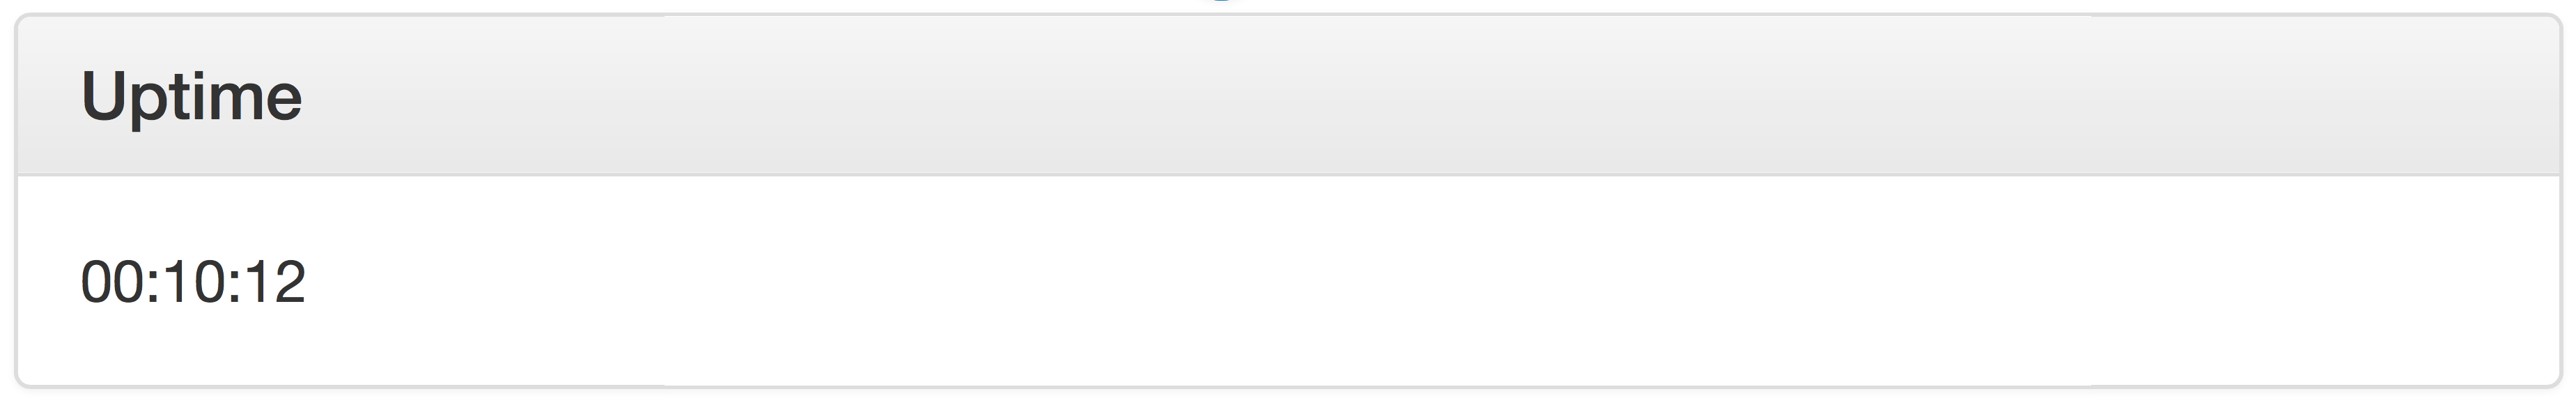
\includegraphics[width=\textwidth]{figures/text.png}
    \caption{Text Element}
    \label{fig:text_element}
\end{figure}

	\item[Checkbox element]
        The checkbox element allows the user to modify a simple boolean value in the model's settings. As an example, it might be used to toggle a certain functionality. Being a control element, it maintains a bi-directional connection with the presenter, so it can notify the presenter whenever a user modifies its value and receive updates whenever another client modifies its associated value. View-presenter interaction will be covered in \cref{sub:presenter_interaction}.

\begin{figure}[H]
  \centering
    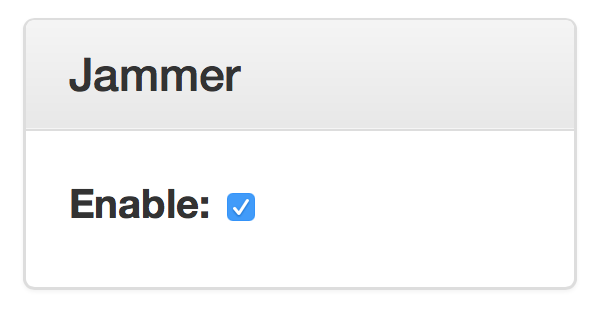
\includegraphics[width=0.3\textwidth]{figures/checkbox.png}
    \caption{Checkbox Element}
    \label{fig:checkbox_element}
\end{figure}

	\item[Slider element]
	A more flexible element that allows to user to set and observe the value of a certain (numerical) parameter in the system. Like the checkbox, this is a control element that is bi-directionally connected to the presenter.

\begin{figure}[H]
    \centering
    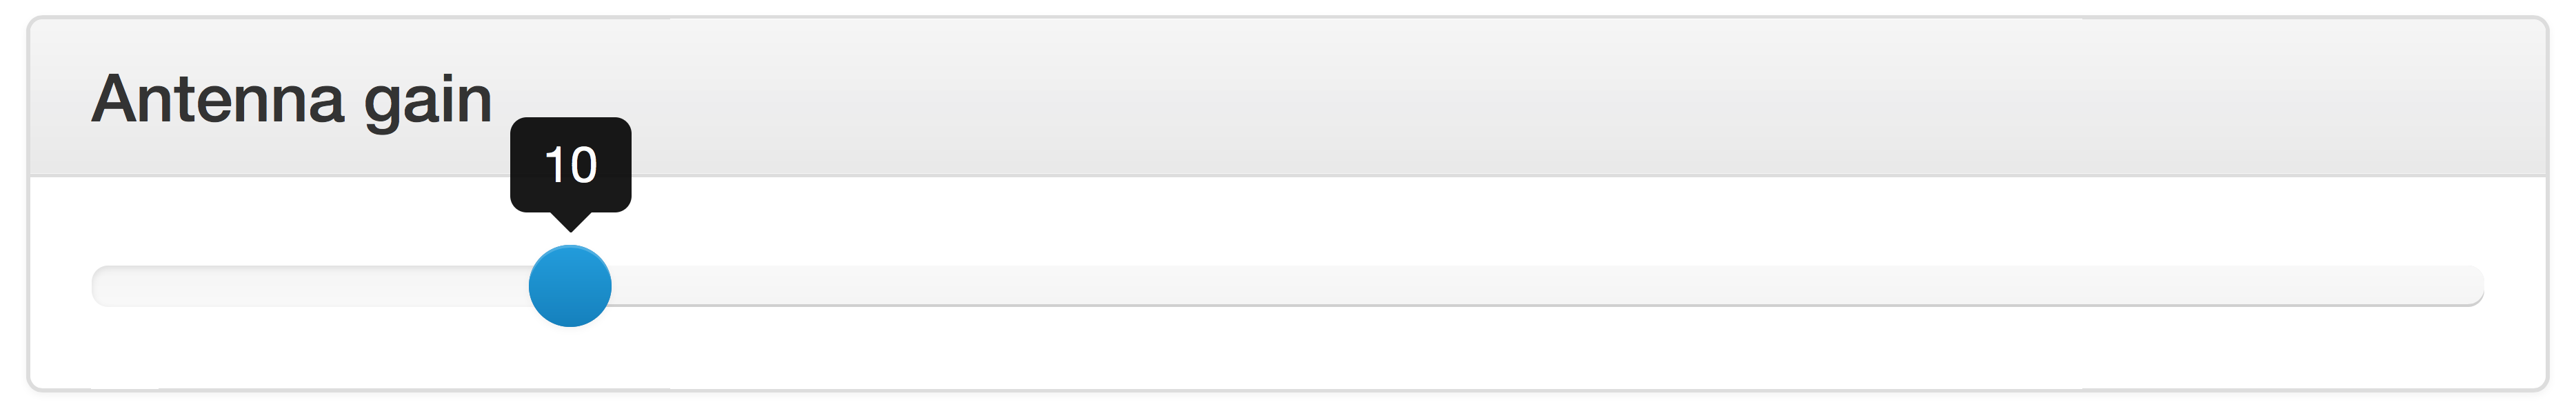
\includegraphics[width=\textwidth]{figures/slider.png}
    \caption{Slider Element}
    \label{fig:slider_element}
\end{figure}

	\item[Visualisation element]
        The last and most complex one available, this element presents the current results of any of the three sub-processes as carried out by the functional core (generation/sampling, reconstruction, detection). The user can pick any of the three datasets to display, which may then be displayed using a real-time spectrogram or an FFT-style plot, or, when detection data is selected, a column diagram that shows at what frequencies an actual signal is determined to be present.
        The spectrogram is developed by our team and allows the user to observe how the frequency spectrum varies over time by depicting a certain frequency content with a certain colour shade.
    The FFT-plots and detection column graphs are generated by the JavaScript plotting library \lib{Highcharts}. The code for both plots mainly consists of setting up \lib{Highcharts} for the correct display of the incoming data, preparing the incoming data for display (apply scaling, etc.) and calculating the correct plot limits to yield a clear picture.
	The FFT-plot is also equipped with averaging functionality, which can be used to smooth the rather variable input data for a more stable image.

\begin{figure}[H]
    \centering
    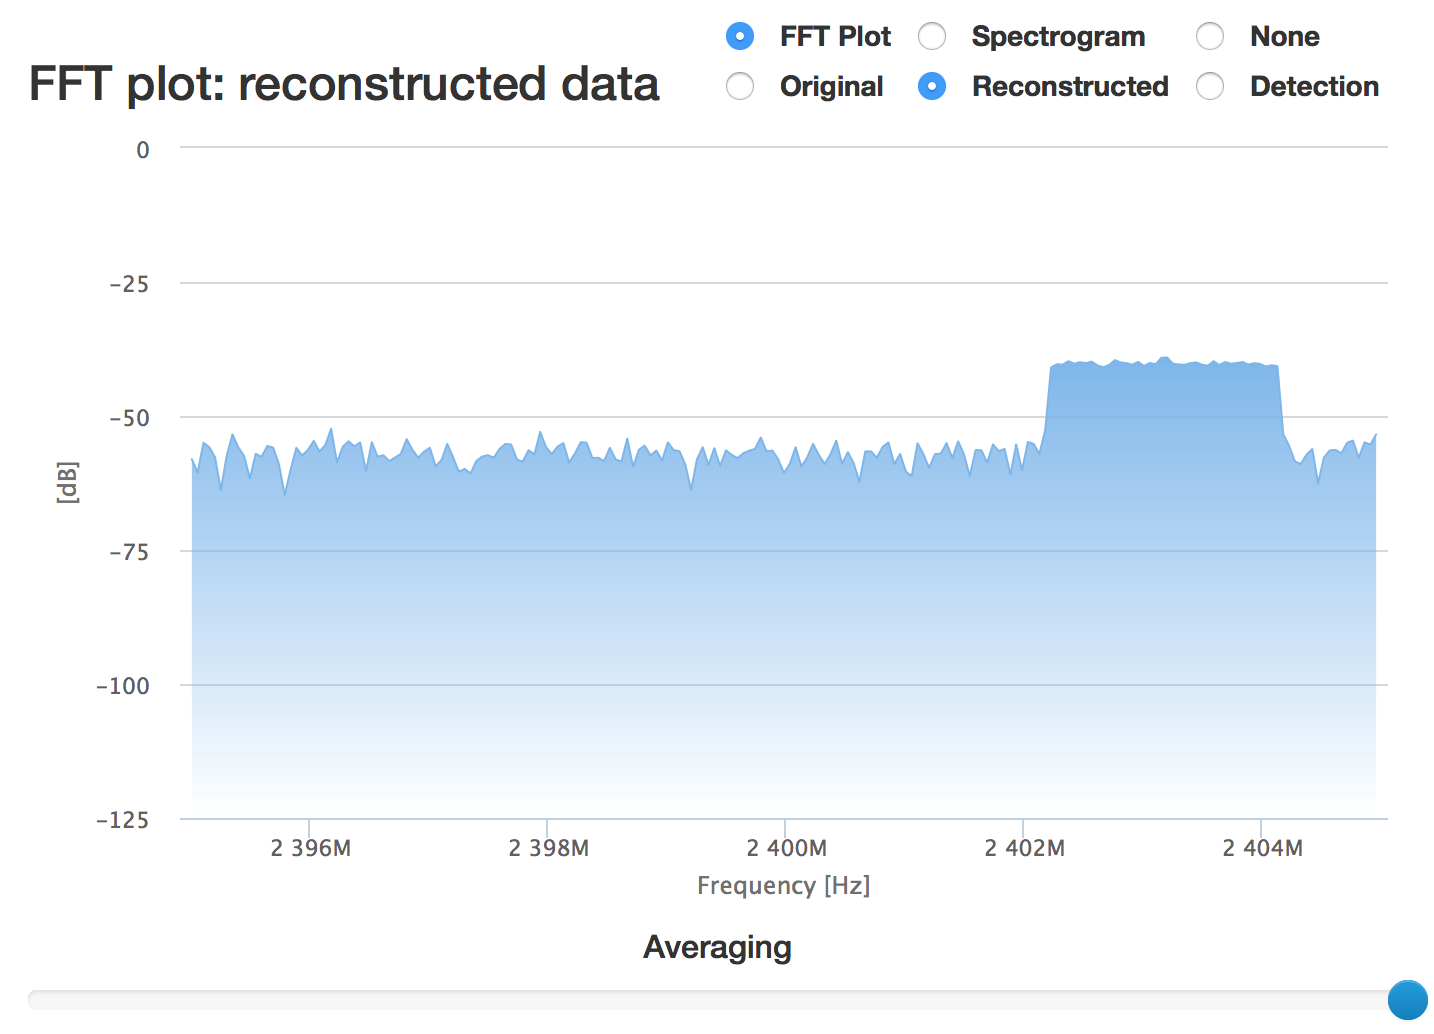
\includegraphics[width=\textwidth]{figures/fft.png}
    \caption{FFT Visualisation Element}
    \label{fig:fft_element}
\end{figure}

\begin{figure}[H]
    \centering
    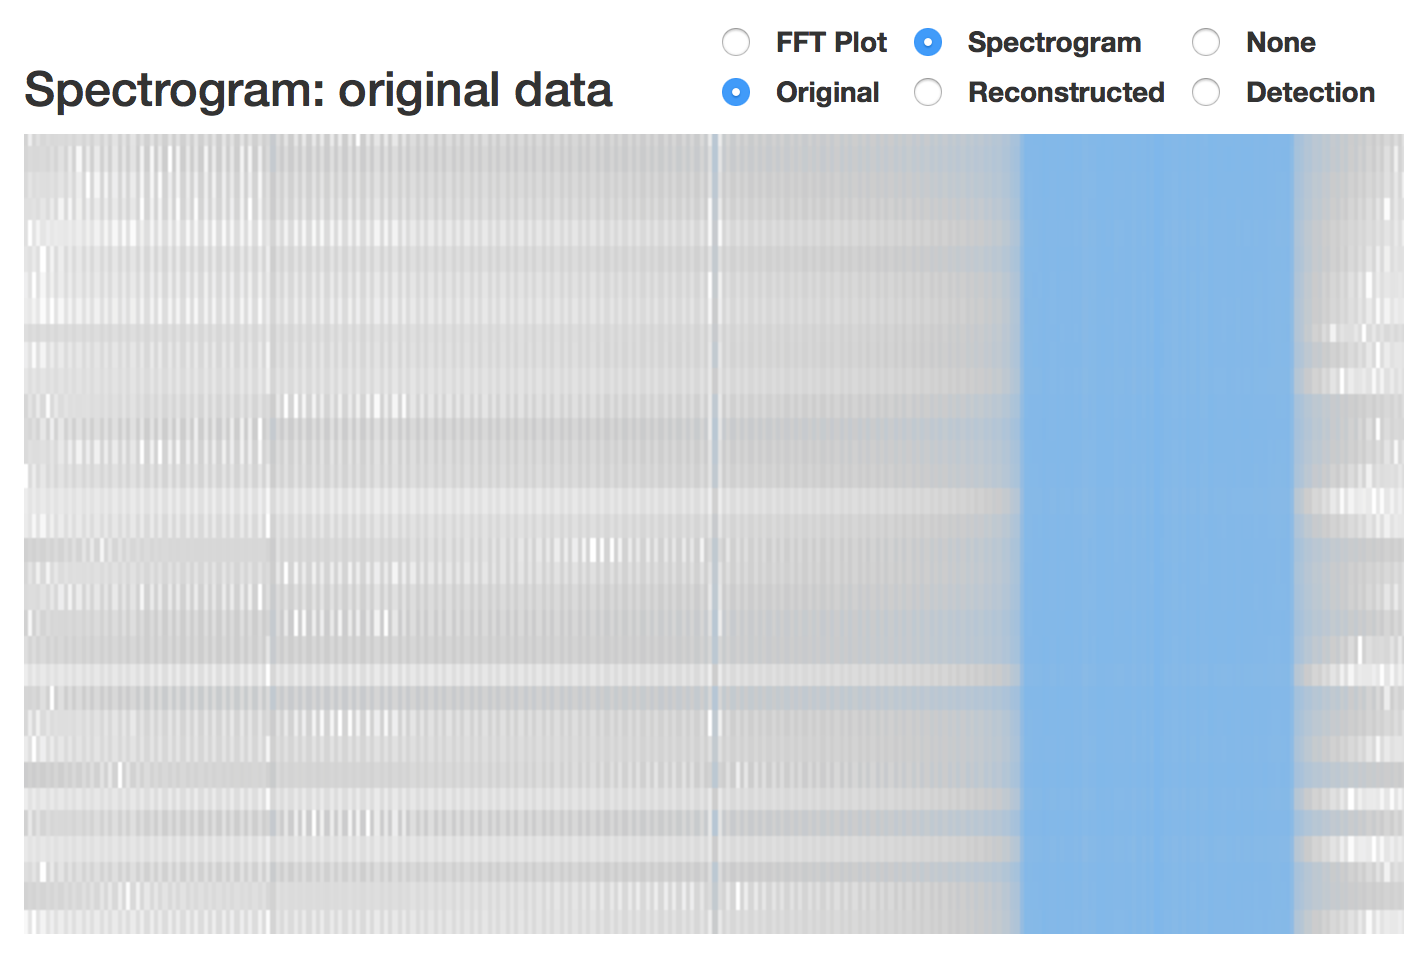
\includegraphics[width=\textwidth]{figures/spectrogram.png}
    \caption{Spectrogram Visualisation Element}
    \label{fig:spectrogram_element}
\end{figure}

\begin{figure}[H]
    \centering
    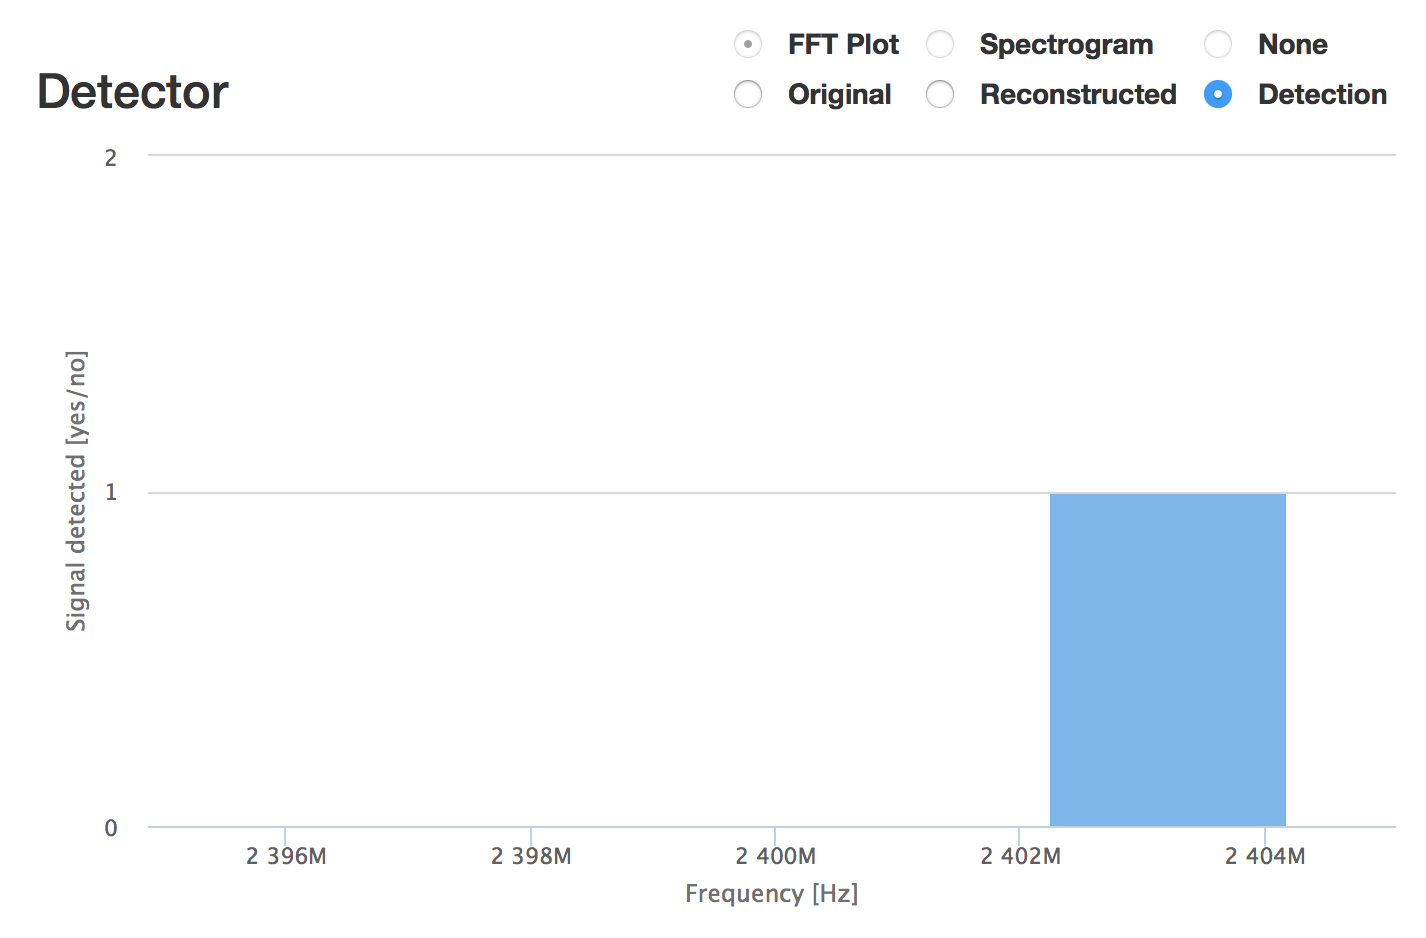
\includegraphics[width=\textwidth]{figures/detection.png}
    \caption{Detection Visualisation Element}
    \label{fig:detection_element}
\end{figure}

\end{description}

Each of the elements consists of server-side and client-side logic, which is written in Python and JavaScript, respectively. The server-side logic consists of a class that contains some of the element's properties, like a unique ID, title and a reference to a \lib{Jinja2} template as previously described, that is rendered whenever the element is used (when the client requests the web application). The client-side logic is a JavaScript object that defines the element's dynamical behaviour, such as handling user-input and/or server-sent updates.

\begin{figure}[H]
    \centering
    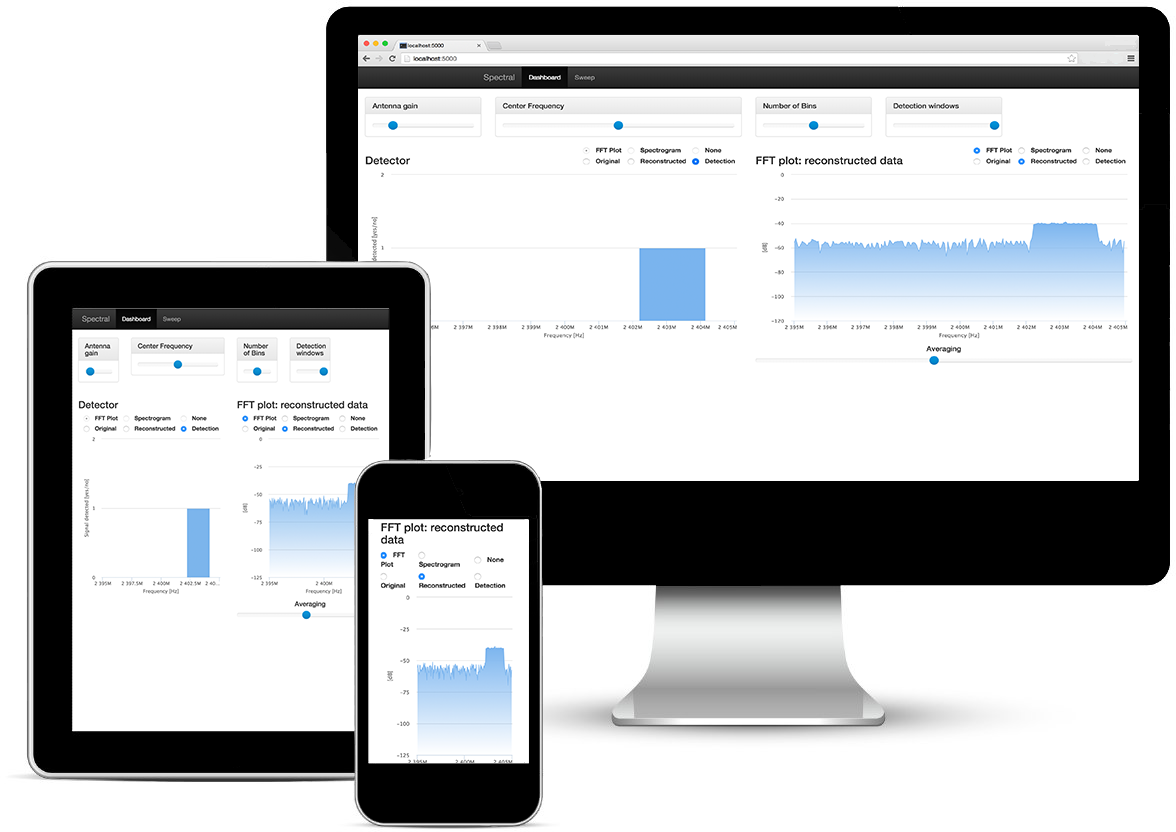
\includegraphics[width=\textwidth]{figures/multidevice.png}
    \caption{The graphical user interface on multiple devices}
    \label{fig:multidevice}
\end{figure}

\cref{fig:multidevice} shows a sample configuration of the view using the described elements on multiple devices.

\section{Front-end}
\label{sec:clientside}
As mentioned, the front-end consists of a web page containing the elements as generated by the server. The user is presented with a certain combination of the elements that were described in the previous section, that allows them to manipulate settings back in the model and verify its results. The front-end is largely based on \lib{Bootstrap}, which provides a solid base to build the rest of the interface on. Bootstrap provides the HTML (HyperText Markup Language, used to define the structure a web page), that defines the grid in which all elements are consequently rendered. Bootstrap also handles the scaling of the entire application for different screen sizes, so the application remains usable, even on smartphones.

\subsection{Presenter interaction}
\label{sub:presenter_interaction}
The model has to be updated upon any user interaction that takes place in the view. At the same time, UI-elements in the view should be able to access the most recent data from the model. For this to happen, a connection has to made between model and view. In \cref{cha:presenter} we introduced the settings and data WebSocket servers, which were built for this goal.

The web application connects to both of these WebSockets using JavaScript's built-in WebSocket implementation, wrapped in the \func{Control} and \\\func{Visualisation} objects, respectively. These two objects are implemented following the \emph{Singleton}-pattern, which is a design-pattern that ensures that only a single instance of the given object may exist at all times (bearing similarities to a \texttt{static} instance of a class in some other languages), which is useful since both \func{Control} and \func{Visualisation} handle all WebSocket related actions for the entire web application \cite[127]{designpatterns}.

The \class{Control} object connects to the settings WebSocket server from \cref{sub:websocket_settings}. Whenever a user modifies a setting, e.g. by altering a slider value, \class{Control} will send a message over the WebSocket to the presenter to notify it of the update.
After this, the presenter will publish the update to the model. The various subcomponents of the model may implement a method to read the most recent system settings that might concern them to process setting updates that might concern the.
The presenter will also broadcast the to all other connected clients. Upon receiving such an update, the \class{Control} object will execute the update routine of the appropriate element, for example moving the slider to the newly received value. This process ensures that the current program settings are synchronised among every client.

The \class{Visualisation} object connects to the data WebSocket server from \cref{sub:websocket_data}. It keeps track of the currently shown data by registering each plot present in the application. Whenever a plot is registered, \class{Visualisation} will send a message over the WebSocket, requesting the presenter to send the current data of the required type. The presenter will respond by sending an object containing the requested data and some additional meta-data. Upon receiving this data, \class{Visualisation} will pass it through to the the element that first triggered the request, which will then re-render the plot. After this, \class{Visualisation} will, again, send a request to the presenter, restarting the cycle. This process will continue until the user picks another data type for display, or disables the plot altogether, which will trigger \class{Visualisation} to unregister the plot and safely destroy it. Carefully keeping track of every plot in the application and the data type it displays like this prevents memory-leaks and bandwidth wasted on unprocessed plot data.

\end{document}
